\subsection{Potential Temperature and Zonal Wind Anomaly}
The zonal-mean potential temperature and potential temperature anomalies for Control, SAI 2020 and SAI 2080 are shown in Figure \ref{fig:th_U_zmdiff_full}, for the annual, JJA and DJF mean. The black countours indicate the zonal-mean zonal wind in m/s. 

In Control we see the potential temperature anomaly signature of increased greenhouse gases, warming at the surface and the troposphere, extending to the lower stratosphere and cooling in the upper stratosphere. The cooling trend in the upper stratosphere is present in SAI 2020 and SAI 2080 as well, but over the Antarctic SAI 2020 and SAI 2080 cool significantly more. With SAI the potential temperature increases where SAI is deployed in the lower stratosphere, conecentrated between 15°S and 30°S around 50 hPa. The warming extends over the Antarctic only in the summer (DJF), because of the lack of incoming solar radiation during the polar night in winter (JJA). The stratosphere in SAI 2020 is about 2.5K warmer than in SAI 2080. The tropospheric temperatures are successfully held at present day values in either SAI scenario, within a margin of $\pm$2.5K.

In JJA (winter) we see that the temperature anomaly in SAI 2020 and SAI 2080 is opposite of the trend in Control. The Antarctic stratosphere cools with SAI instead of warming as it does under global warming. In DJF (summer) the anomaly is much more comparable, with warming over the Antarctic in all scenarios.

The zonal winds are mostly driven by the meridional temperature gradient through the thermal wind balance. Qualitatively, we see in Reference that the subtropical jet (STJ) in the lower stratosphere forms above a steep meridional temperature gradient around 30°S.

We also see an increase in wind speed around 50°S where we would expect to see the eddy-driven jet (EDJ), also above a relatively steep meridional gradient. From the wind speeds alone it seems the EDJ is weaker than the STJ, however, we know that the EDJ is generally stronger. This is because of the waviness of the EDJ, so clear identification must follow from eddy-activity, covered in Section \ref{EDJ_sec}. 

Because the STJ and EDJ and their anomalies are strongest in winter, we will focus on this season in any further analysis of these jets in the lower stratosphere.

In the upper stratosphere we see in JJA a strong westerly wind, the polar night jet (PNJ). Comparison of the winter and summer meridional temperature gradient reveals that this jet is driven by temperature gradients as well. The meridional temperature gradient is positive (equator-to-pole) in JJA, resulting in strong westerlies. In DJF the gradient flattens in the stratosphere – even turning slightly negative in the upper stratosphere - preventing strong westerly winds from forming. 

In all scenarios the PNJ shifts equatorward, in Control because the latitude of the highest temperature gradient shifts over the whole stratosphere, in SAI 2020 and SAI 2080 because the temperature gradient strongly increases on the equatorward side in the lower stratosphere. This will be discussed in more detail in Section \ref{upperstrat}.

\begin{figure}[H]
	\centering
	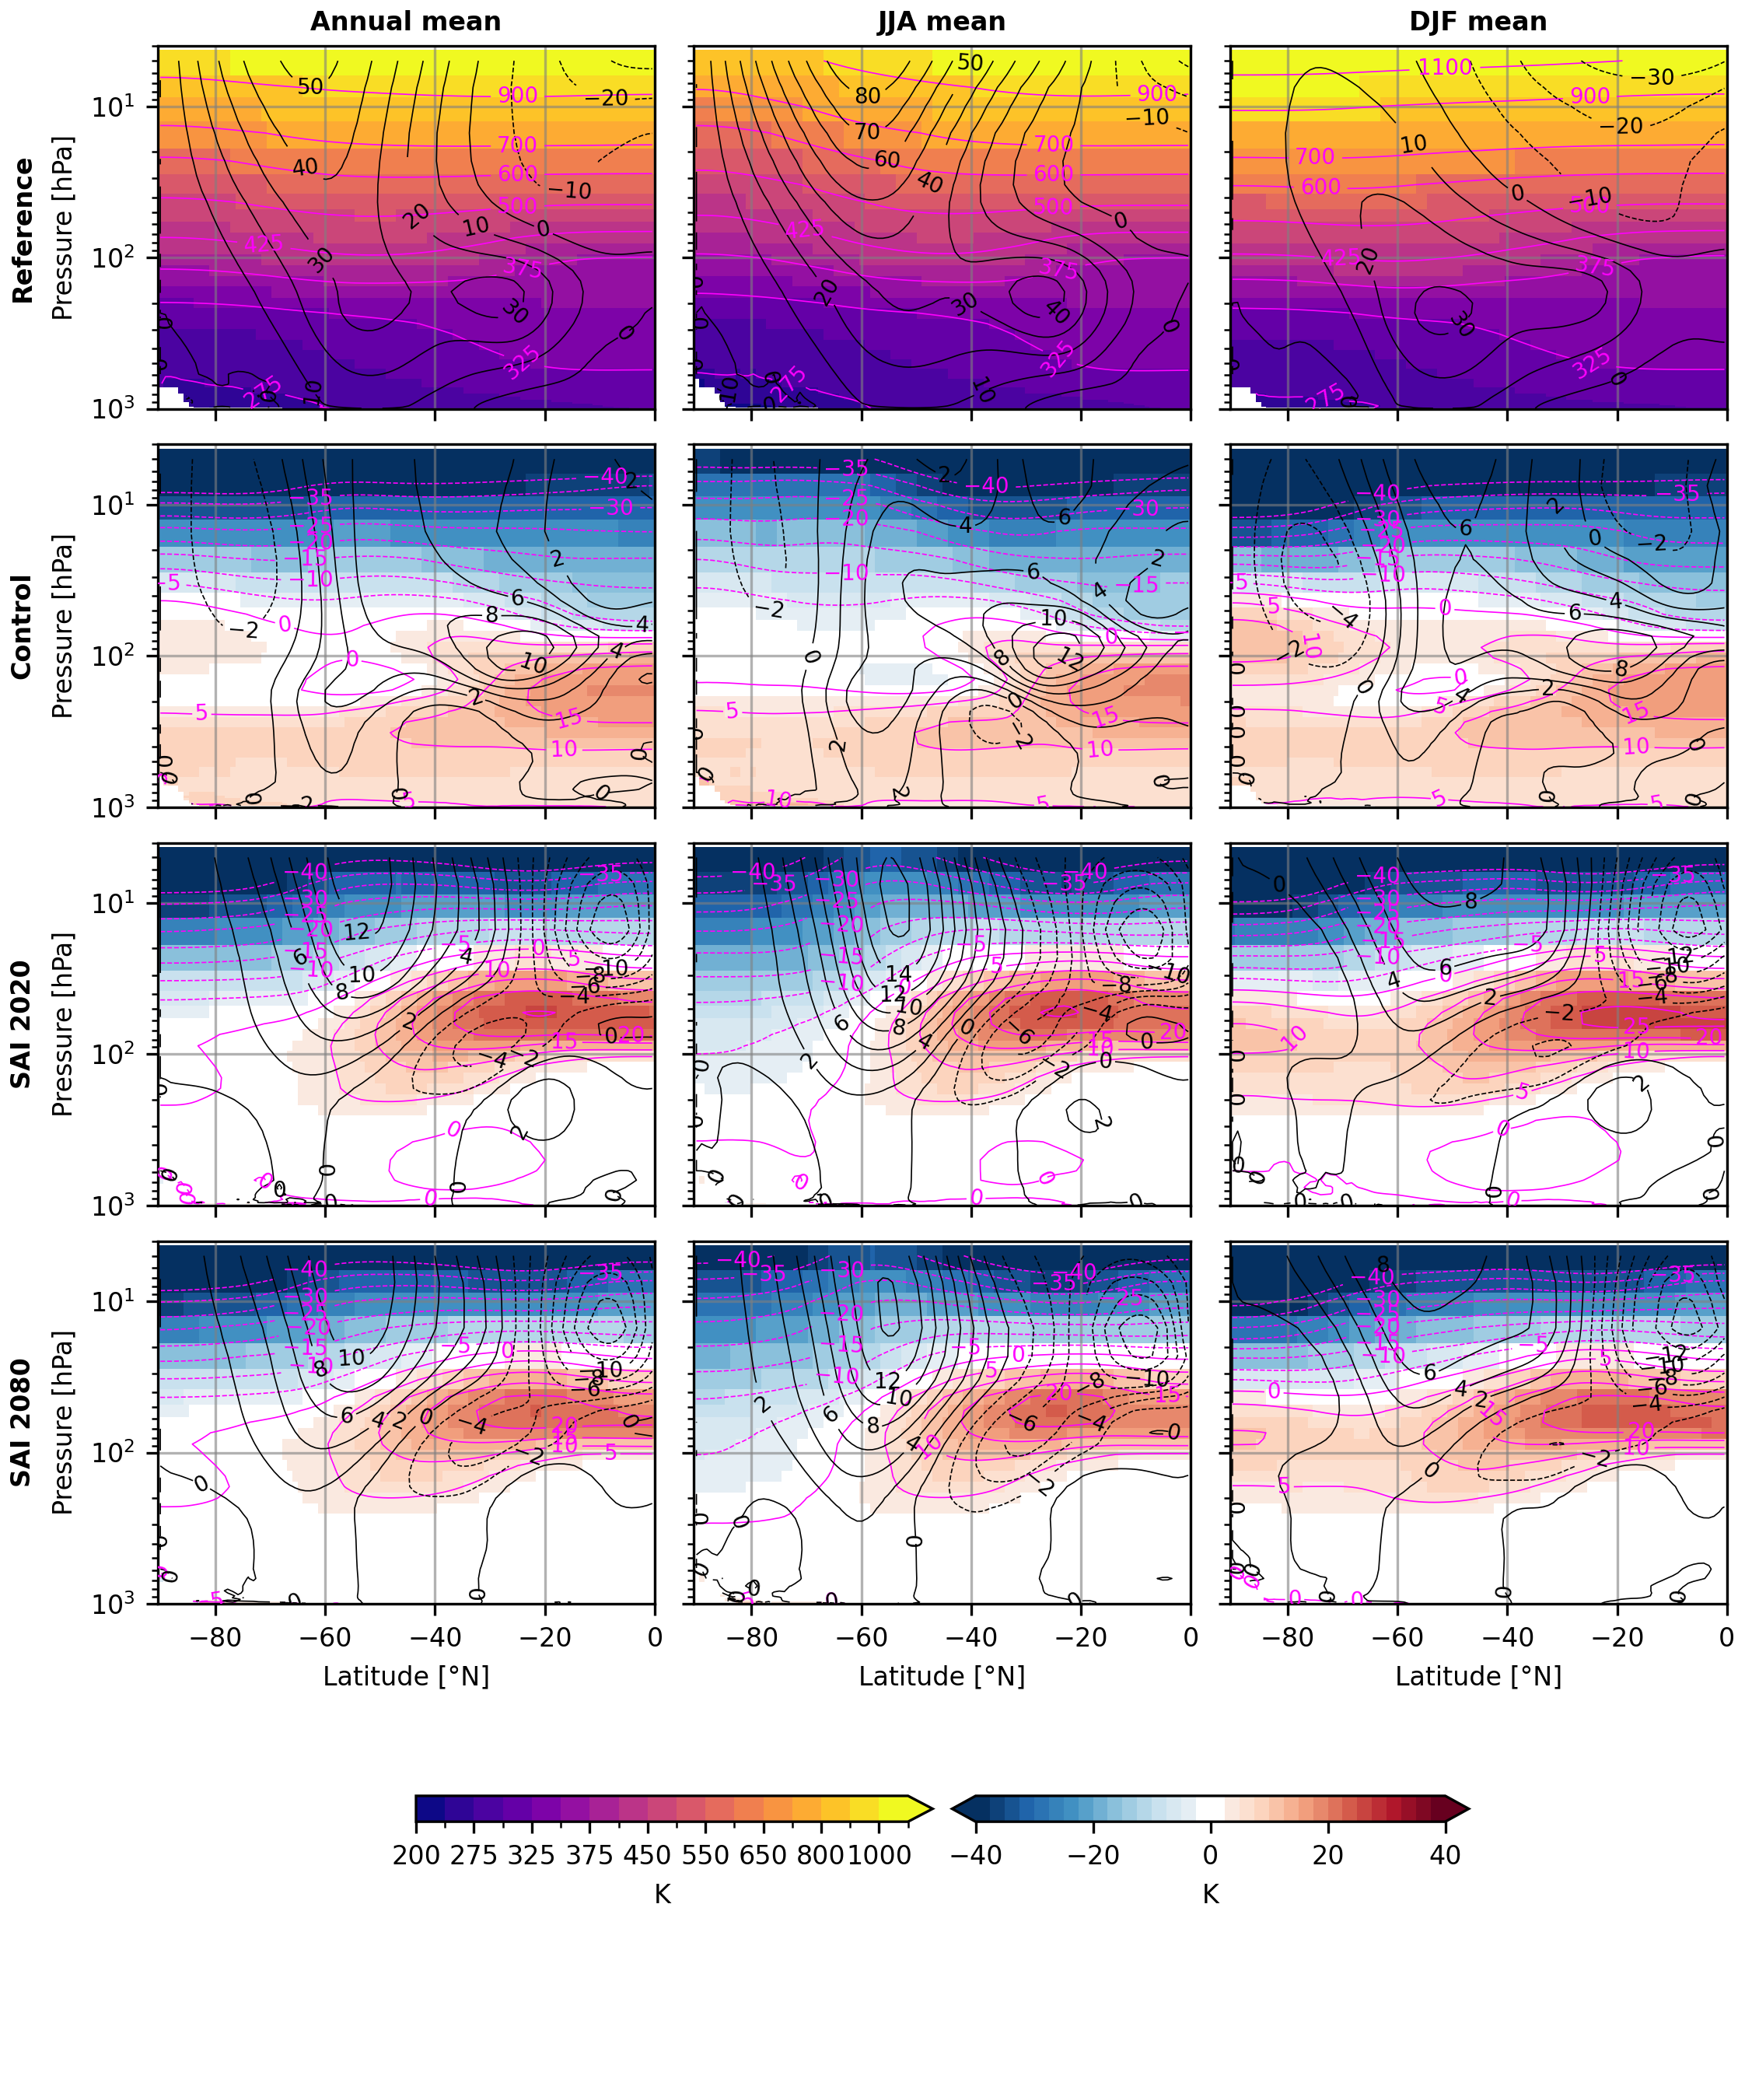
\includegraphics[width=\linewidth]{images/th_U_zmdiff_full.png}
	\caption{Annual and seasonal mean zonal-mean potential temperature (shading and magenta contours) and zonal-mean zonal wind (black contours, m/s) for Reference (first row) and Control, SAI 2020 and SAI 2080 anomaly compared to Reference (second to fourth row).}
	\label{fig:th_U_zmdiff_full}
\end{figure}

\subsection{Results Part II: Lower Stratosphere}\label{lowerstrat}

\subsubsection{Subtropical Jet}
In Figure \ref{fig:th_U_zmdiff_full} the zonal mean of the zonal component of the integrated thermal wind is shown, together with the observed zonal-mean zonal wind in black countours. The observed wind and integrated thermal wind show a strikingly similar pattern, with the observed wind consistently lower than the integrated thermal wind due to friction effects, increasingly so further up in the atmosphere. 

The change in magnitude of the lower stratosphere wind strongly correlates with the change in magnitude of the integrated thermal wind. The STJ shifts upward and equatorwad in Control, also showing a significant increase of up to 12 m/s in the upper regions. This pattern is consistent with the change in potential temperature in Figure \ref{fig:th_U_zmdiff_full}. See also Figure \ref{fig:th_U_zm_JJA} in Appendix \ref{app_th_U_JJA}, the meridional gradient of the 350K isotherm is much steeper around 30°S in Control compared to Reference.

In contrast, in both SAI 2020 and SAI 2080 the STJ decreases in strength, up to 6 m/s in the upper regions around 100 hPa. This possibly also indicates an equatorward shift, but slightly downward instead of upward. 

\begin{figure}[H]
	\centering
	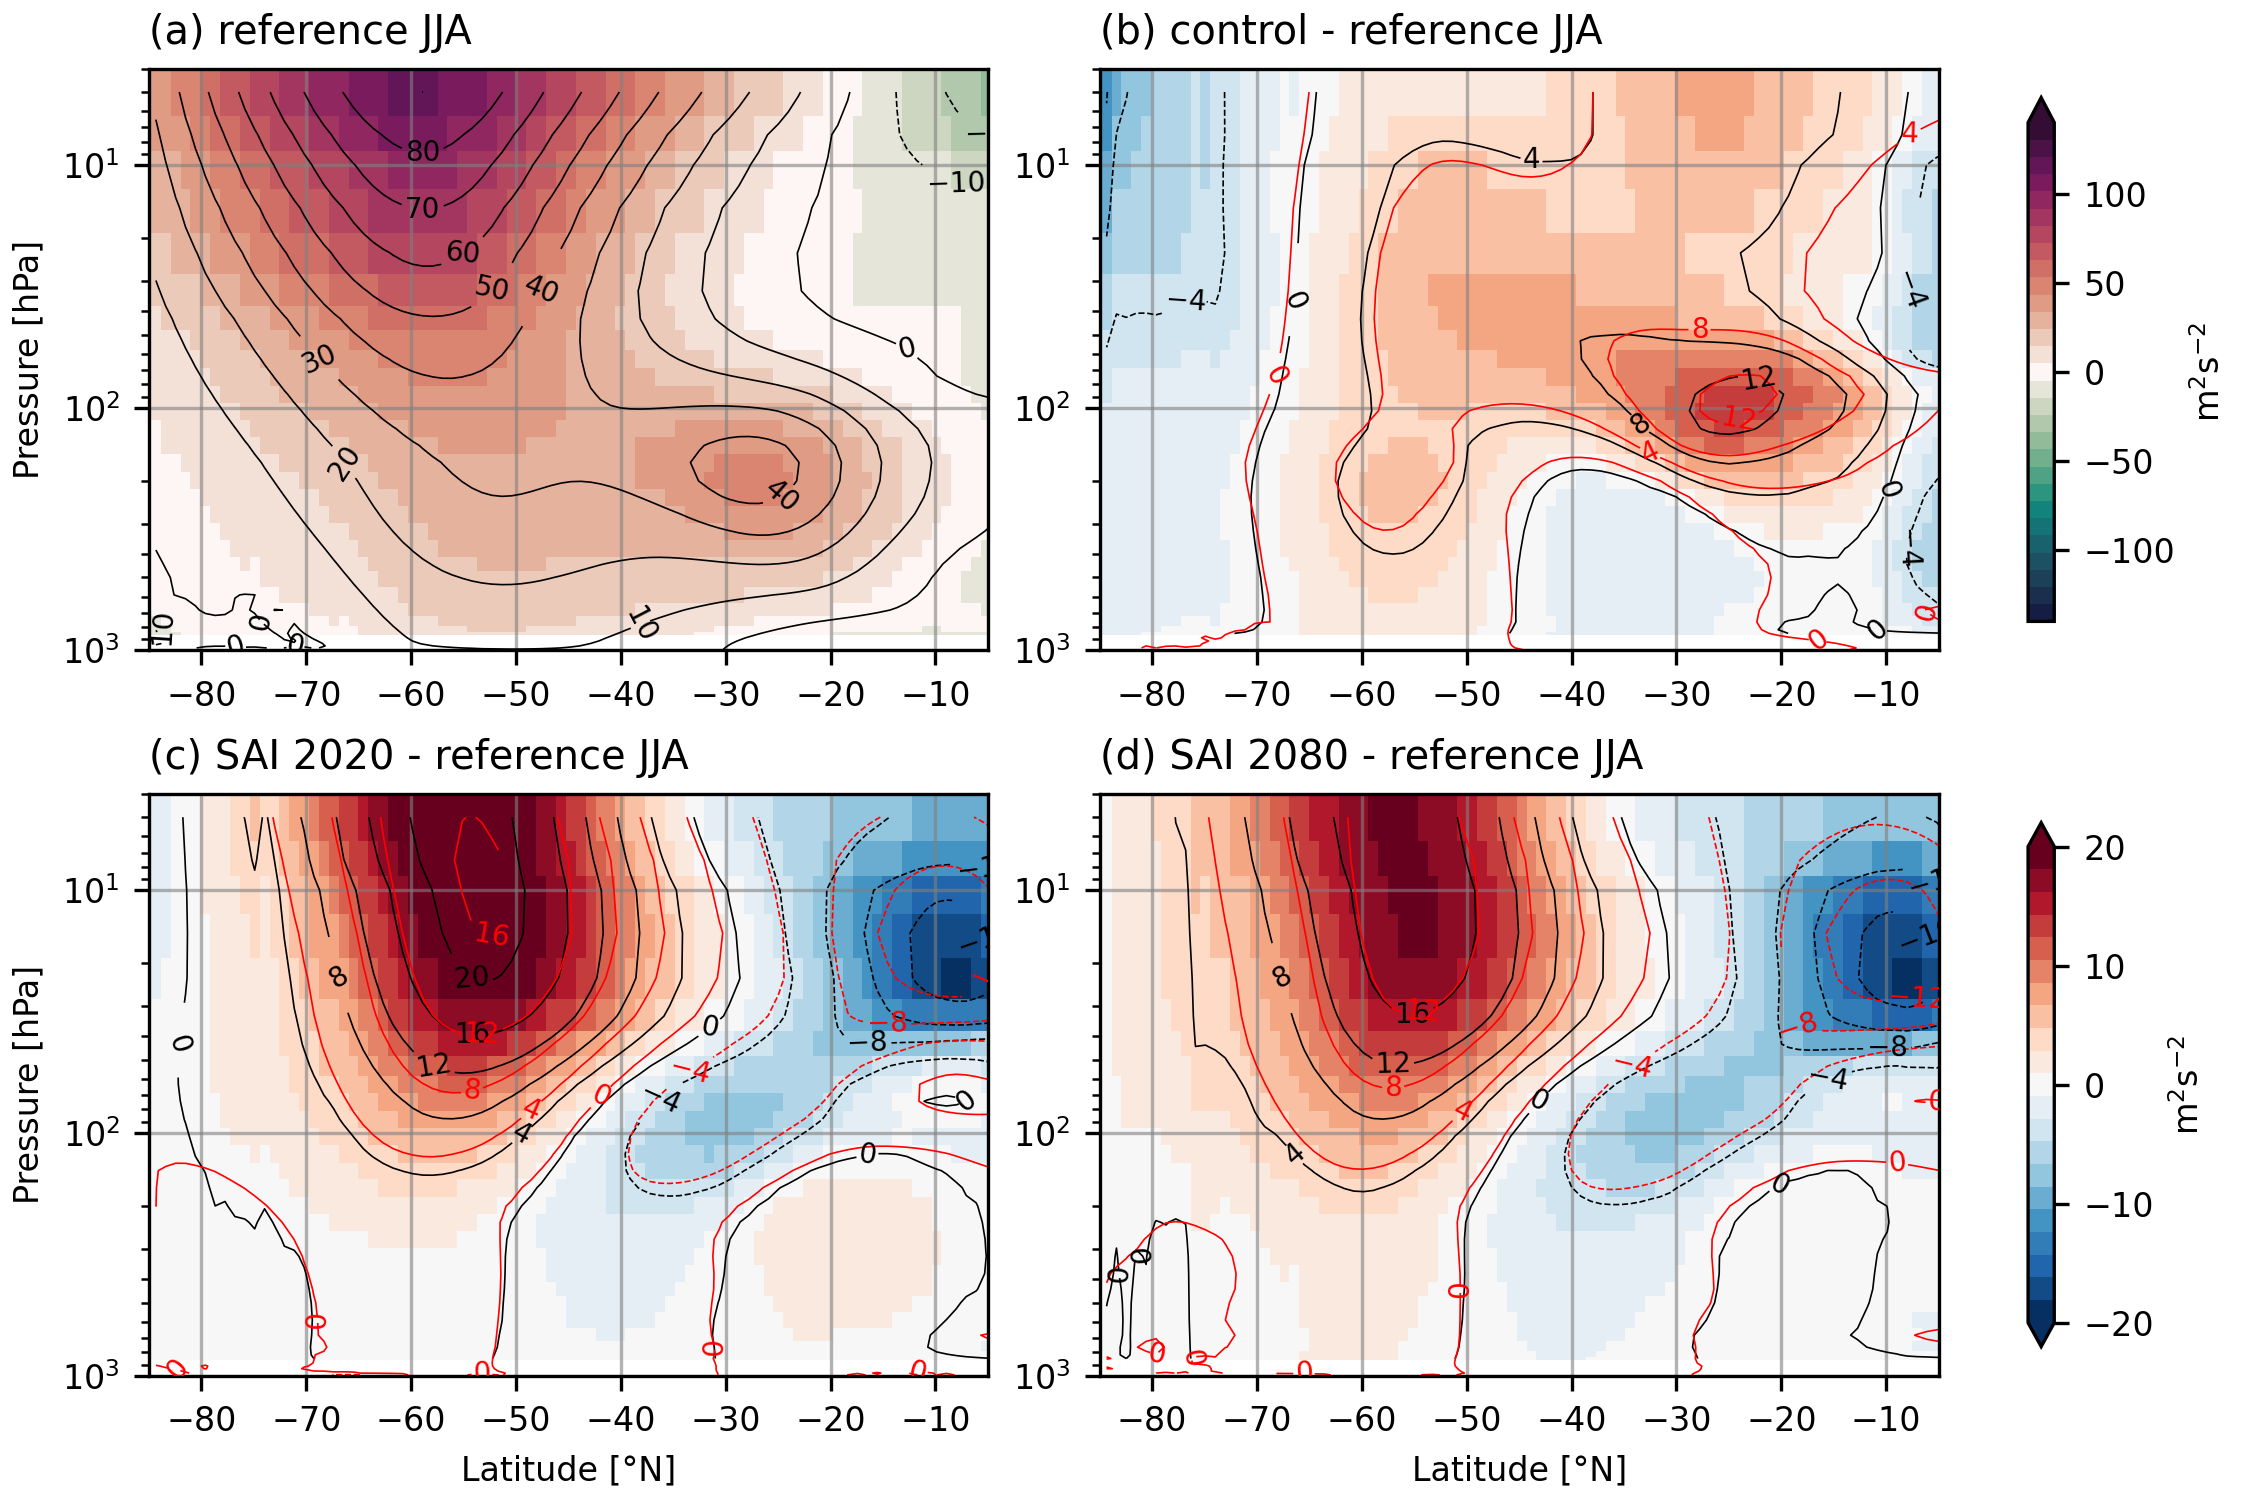
\includegraphics[width=0.95\linewidth]{images/UT_U_zmdiff_JJA.png}
	\caption{JJA mean zonal-mean zonal thermal wind (shading and red contours) and zonal-mean zonal wind (black contours, m/s) for (a): Reference; (b-d): Control, SAI 2020 and SAI 2080 anomaly compared to Reference.}
	\label{fig:UT_U_zmdiff_JJA}
\end{figure}

On the subtropical jet intensity map in Figure \ref{fig:STJ_map_JJA} the same trends as above are observed. In Control the jet intensifies and shifts equatorward. The largest increase is observed in the eastern Pacific Ocean, in Reference the jet is relatively weak in this region, but in Control the jet is the at its peak here. The area between 120°W and 60°E increases the most relatively, the opposite hemisphere shows little change.

In SAI 2020 and SAI 2080 the jet is much less intense, but the spatial distribution remains largely unchanged. The jet weakens slightly more in SAI 2080 than in SAI 2020, but the difference does not seem significant. 

The location, height and mean of the maximum of the STJ reported in Figure \ref{fig:STJ_maxloc_JJA} largely confirm the patterns observed above. In Control, the STJ maximum shifts equatorwad between 120°W and 60°E and remains around the position of Reference in the other hemisphere, correlating to the increase in intensity. The upward shift of the maximum is about 25 hPa, and the mean maximum wind speed increases 6.2 m/s, or 12.7\%. 

The maximum wind speed in SAI 2020 and SAI 2080 remains mostly at Reference levels, deviating at most 1.1 m/s, or 2\%, in SAI 2020 which is not significant. As the maximum wind speed does not change considerably, but the jet does appears much less intense, this means the jet has become more constrained without losing much strength at its maximum. The location of the maximum in SAI 2020 and SAI 2080 has not shifted much overall, only significantly around 60°E. Looking at the intensity in Figure \ref{fig:STJ_map_JJA} this seems to be the result of the wind speeds in the eddy-driven jet (around 50°S) reaching similar levels as the STJ jet. The EDJ effectively competes with the STJ for the maximum wind speed and `wins' a considerable amount of times.


\begin{figure}[H]
	\centering
	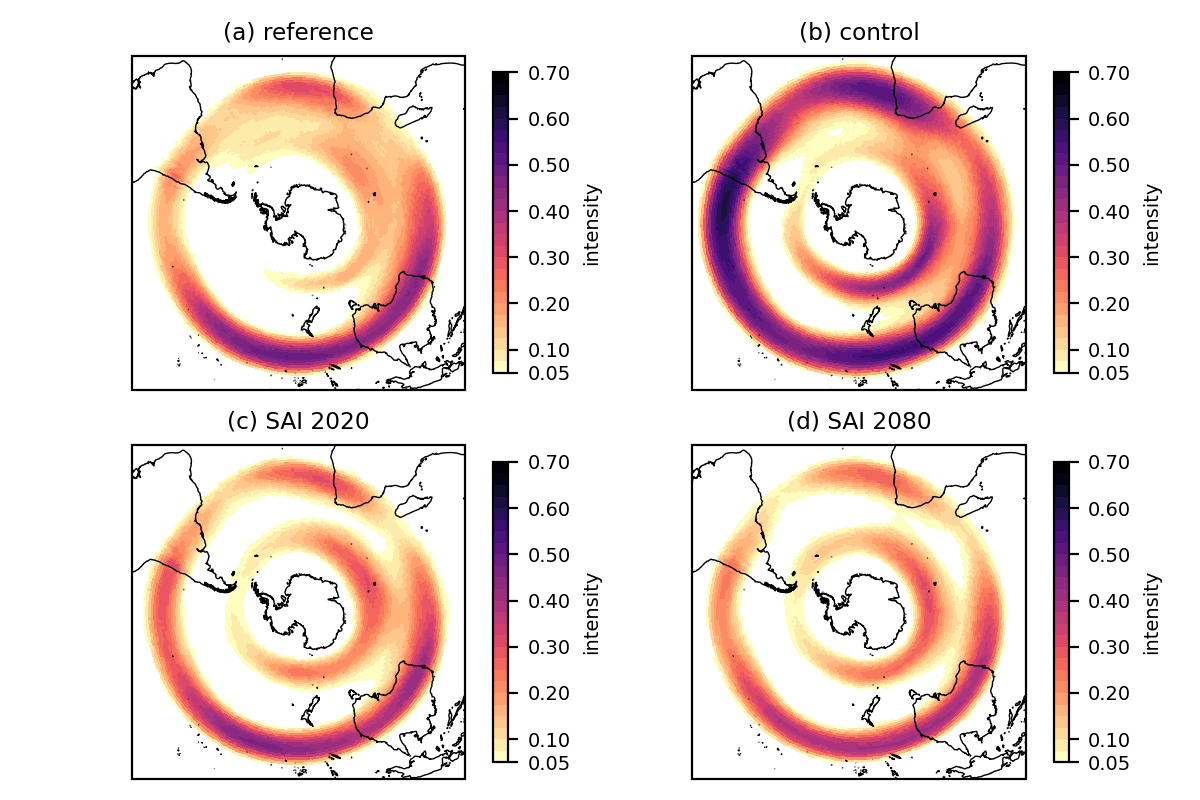
\includegraphics[width=0.95\linewidth]{images/STJ_map_JJA.png}
	\caption{JJA subtropical jet intensity map of zonal wind, values counted when the threshold of 40 m/s was passed between 400 and 100 hPa, for (a) Reference, (b) Control, (c) SAI 2020 and (d) SAI 2080. 0°E is oriented towards the top of the figure.}
	\label{fig:STJ_map_JJA}
\end{figure}

\begin{figure}[H]
	\centering
	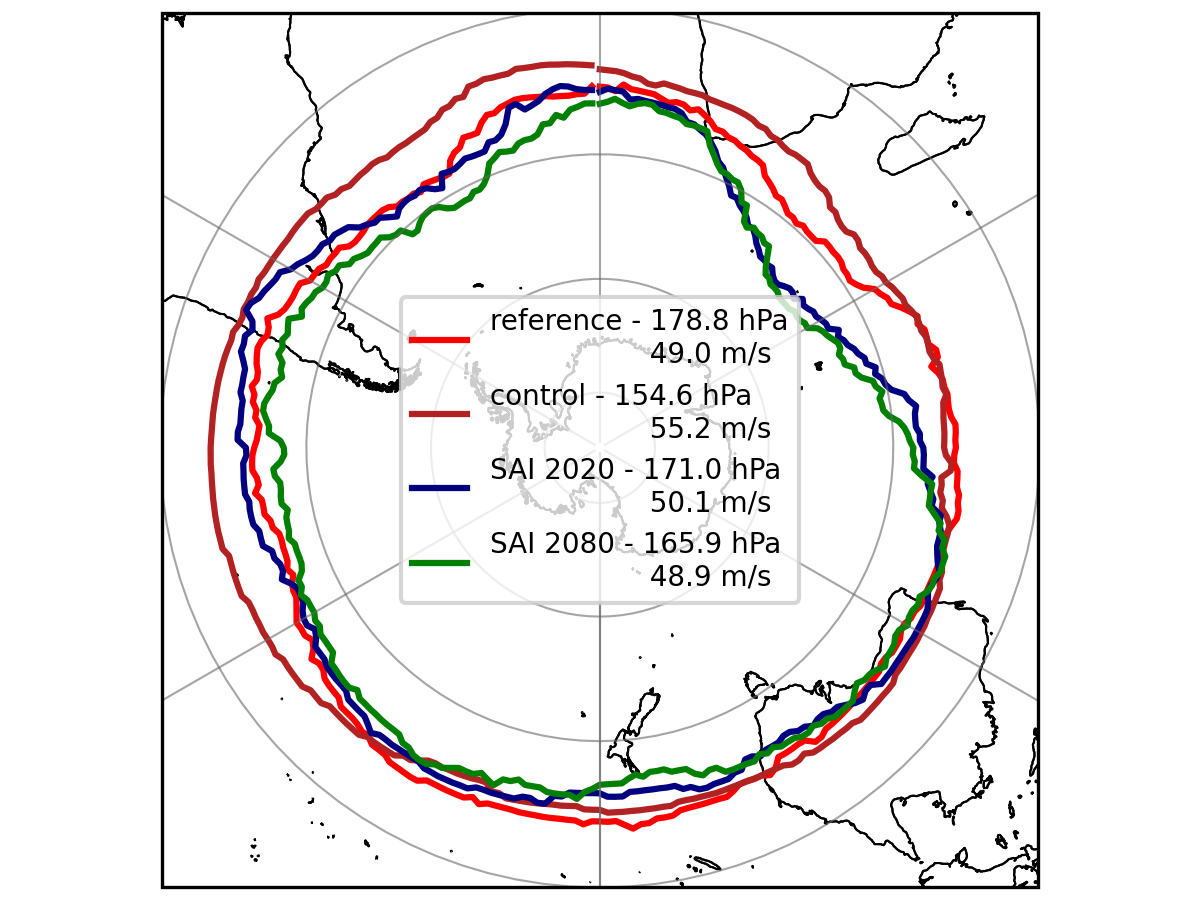
\includegraphics[width=0.48\linewidth]{images/STJ_maxloc_JJA.png}
	\caption{JJA mean location of the maximum of the subtropical jet, with corresponding longitudinal mean height and maximum eddy kinetic energy for Reference, Control, SAI 2020 and SAI 2080. 0°E is oriented towards the top of the figure.}
	\label{fig:STJ_maxloc_JJA}
\end{figure}


\subsubsection{Eddy-driven Jet}\label{EDJ_sec}
The EDJ is already visible in Figure \ref{fig:STJ_map_JJA}. The zonal wind in the Eastern Hemisphere reveals another jet structure next to the STJ. Beacuse this jet is driven by eddy activity, the zonal wind alone will not reveal much on its behaviour. We use eddy kinetic energy (EKE) as a measure for eddy activity. The zonal-mean EKE and EKE anomalies are shown in Figure \ref{fig:EKE_U_zmdiff_JJA}.

Around 50°S and 300 hPa, there is a peak in EKE, i.e. high eddy activity, this is where we identify the EDJ to be. In Control the EKE decreases on the lower equatorward side of the jet and increases on the upper poleward side, indicating that the jet shifts poleward and upward. It is not clear from this figure if the jet becomes more or less wavy. In SAI 2020 and SAI 2080 the EKE shows small changes compared to what is observed in Control. A slight decrease is observed around 45°S, in the area between the EDJ and the STJ, and stays close to Referene levels everywhere else. SAI 2020 responds more strongly than SAI 2080.

The eddy-driven jet intensity map in Figure \ref{fig:EDJ_map_JJA} also indicates an increase in intensity in Control and a poleward shift. The change in intensity in SAI 2020 and SAI 2080 is again much smaller, both weakening slightly while the overall spatial pattern remains largely unchanged. 

The location of the maximum in Figure \ref{fig:EDJ_maxloc_JJA} reveals that the EDJ remains largely in position in both SAI scenarios, but shifts poleward everywhere in Control. The upward shift identified in Figure \ref{fig:EKE_U_zmdiff_JJA} in Control is confirmed to be about 23 hPa. In SAI 2020 and SAI 2080 the jet maximum shifts slightly downward, though not significantly. In each scenario the mean maximum EKE decreases slightly but insignificantly, 2-4\%, again not providing much insight into any changes waviness of the jet. 

\begin{figure}[H]
	\centering
	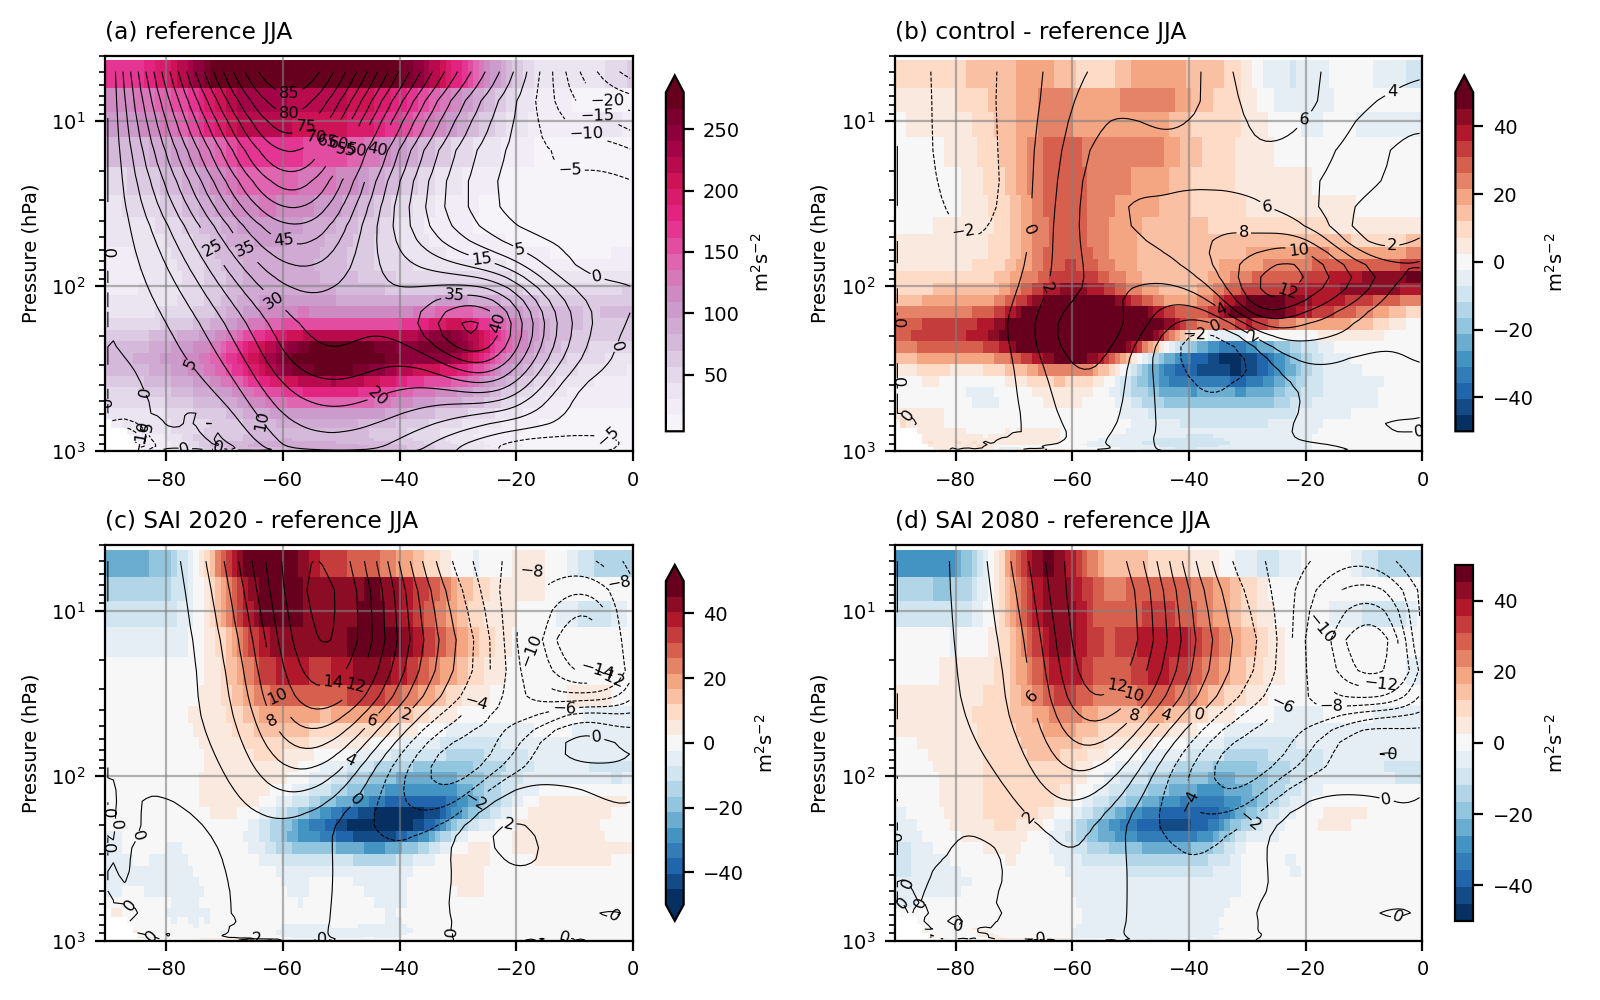
\includegraphics[width=0.95\linewidth]{images/EKE_U_zmdiff_JJA.png}
	\caption{JJA mean zonal-mean eddy kinetic energy (shading) and zonal-mean zonal wind (contours, m/s) for (a): Reference; (b-d): Control, SAI 2020 and SAI 2080 anomaly compared to Reference.}
	\label{fig:EKE_U_zmdiff_JJA}
\end{figure}

\begin{figure}[H]
	\centering
	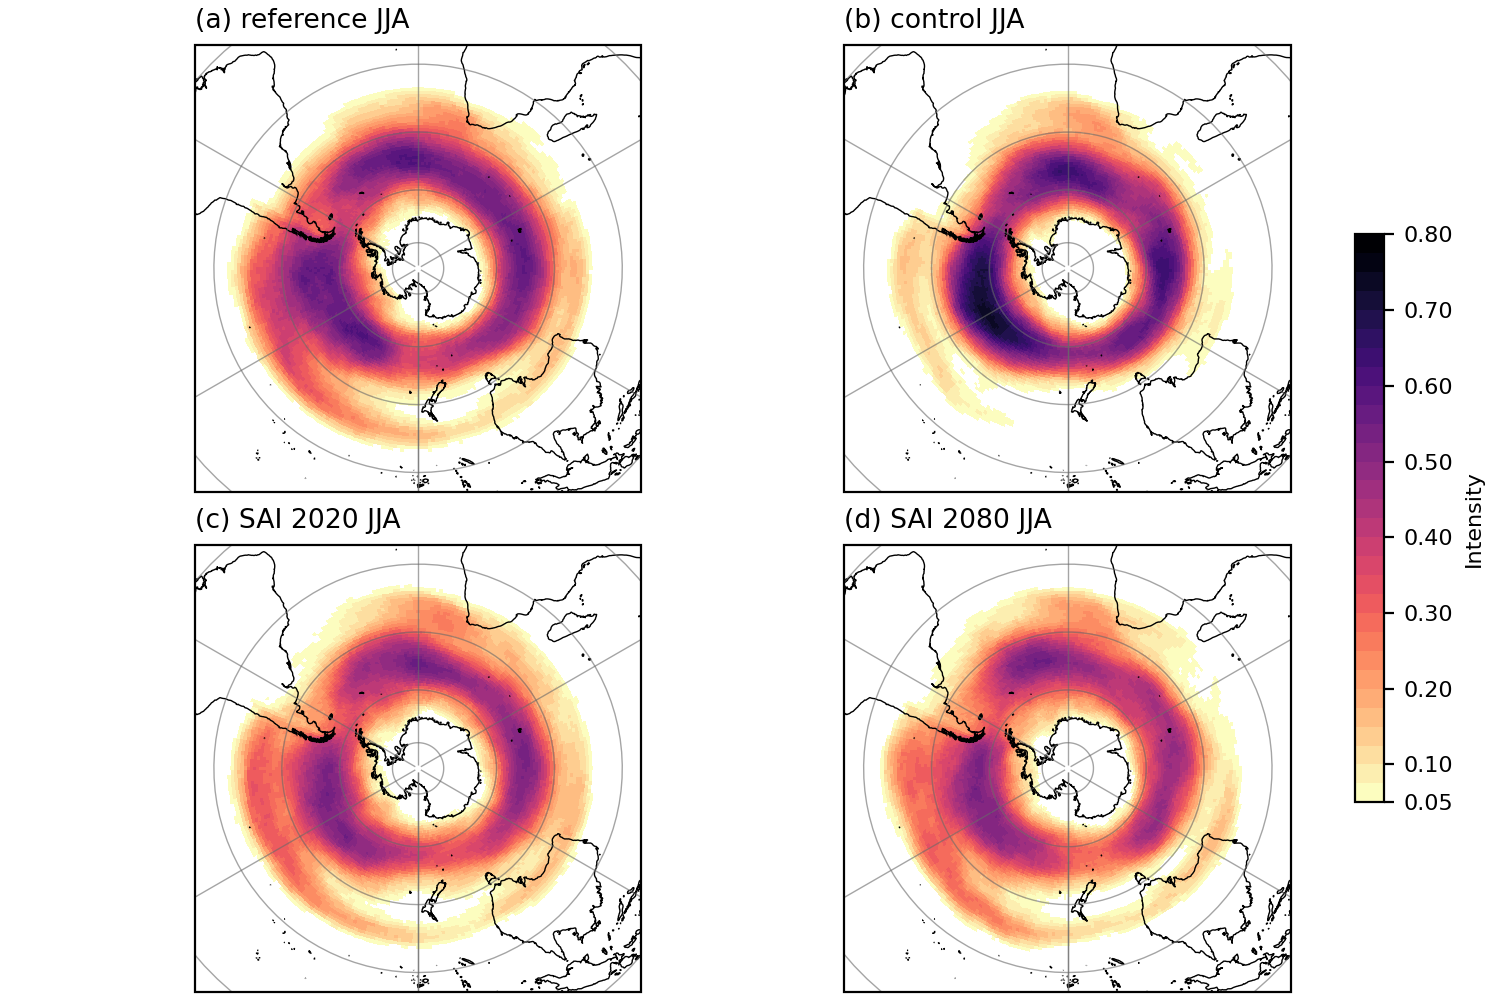
\includegraphics[width=0.95\linewidth]{images/EDJ_map_JJA.png}
	\caption{JJA eddy-driven jet intensity map of EKE, values counted when the threshold of 105 J/m$^3$ was passed between 600 and 150 hPa, for (a) Reference, (b) Control, (c) SAI 2020 and (d) SAI 2080. 0°E is oriented towards the top of the figure.}
	\label{fig:EDJ_map_JJA}
\end{figure}

\begin{figure}[H]
	\centering
	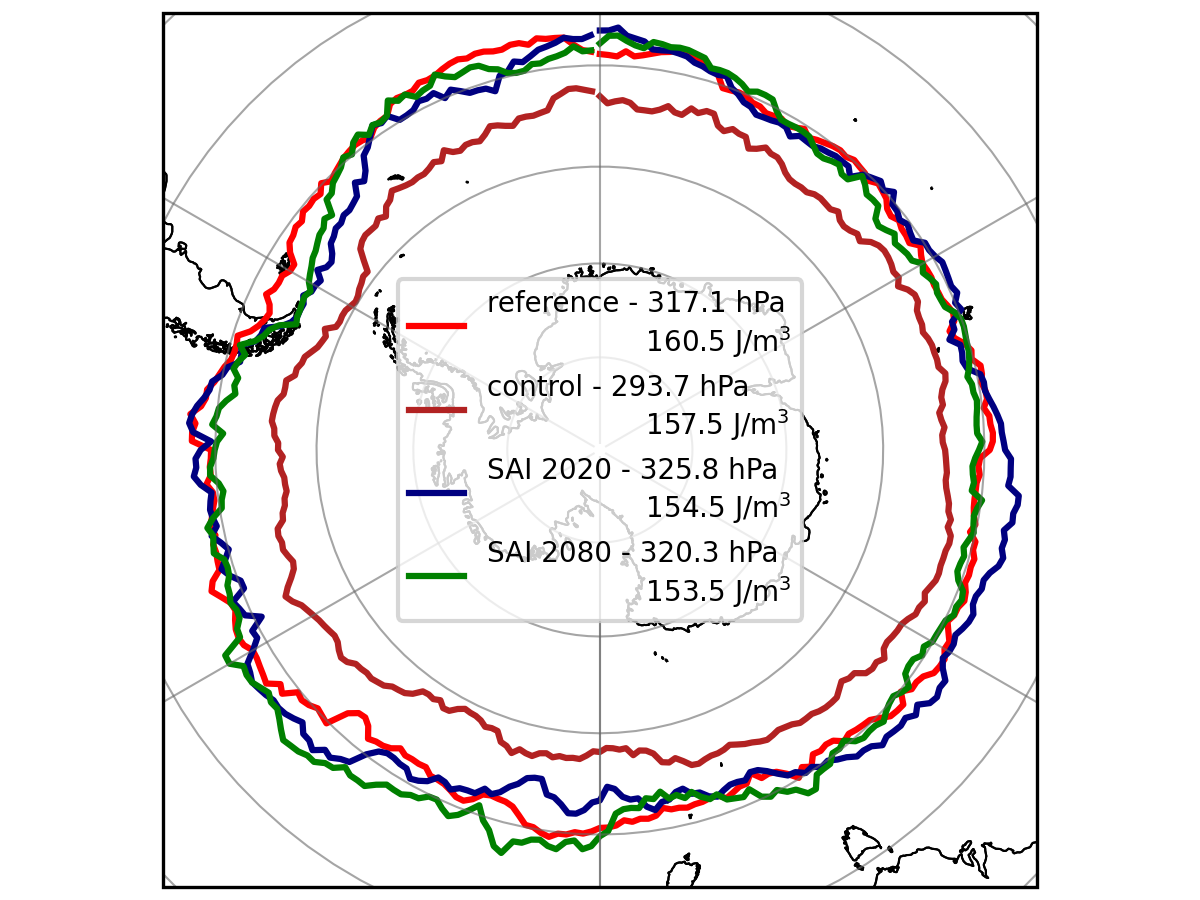
\includegraphics[width=0.48\linewidth]{images/EDJ_maxloc_JJA.png}
	\caption{JJA mean location of the maximum of the eddy-driven jet, with corresponding longitudinal mean height and maximum eddy kinetic energy for Reference, Control, SAI 2020 and SAI 2080. 0°E is oriented towards the top of the figure.}
	\label{fig:EDJ_maxloc_JJA}
\end{figure}
\newpage
The STJ has more kinetic energy than the EDJ, mostly because of the higher mean wind speeds. The EDJ has a proportionally larger eddy component and thus higher EKE. Comparing the changes in KE and EKE and zonal wind speed
will provide insight into the waviness of the two jets. 

In Figure \ref{fig:KE_U_zmdiff_JJA} the zonal-mean kinetic energy and zonal-mean zonal wind are shown. In Control the increase in KE follows the zonal wind patterns in sign and in magnitude. The KE increases with the increasing zonal wind accordingly in the upper regions of the STJ and decreases proportionally below. The KE also increases proportionally to wind speed in the EDJ. This indicates that the STJ and the EDJ do not become siginificantly more or less wavy under global warming.

For SAI 2020 and SAI 2080 the KE anomaly follows the zonal wind anomaly proportionally as well. Comparison with Figure \ref{fig:EKE_U_zmdiff_JJA} shows that the decrease in EKE for the EDJ is correlated with the decrease in zonal wind. The decrease in KE in the STJ shows that the constraining of the jet observed in Figure \ref{fig:STJ_map_JJA} leads to a loss of strength, even while maintaining maximum wind speed.


\begin{figure}[H]
	\centering
	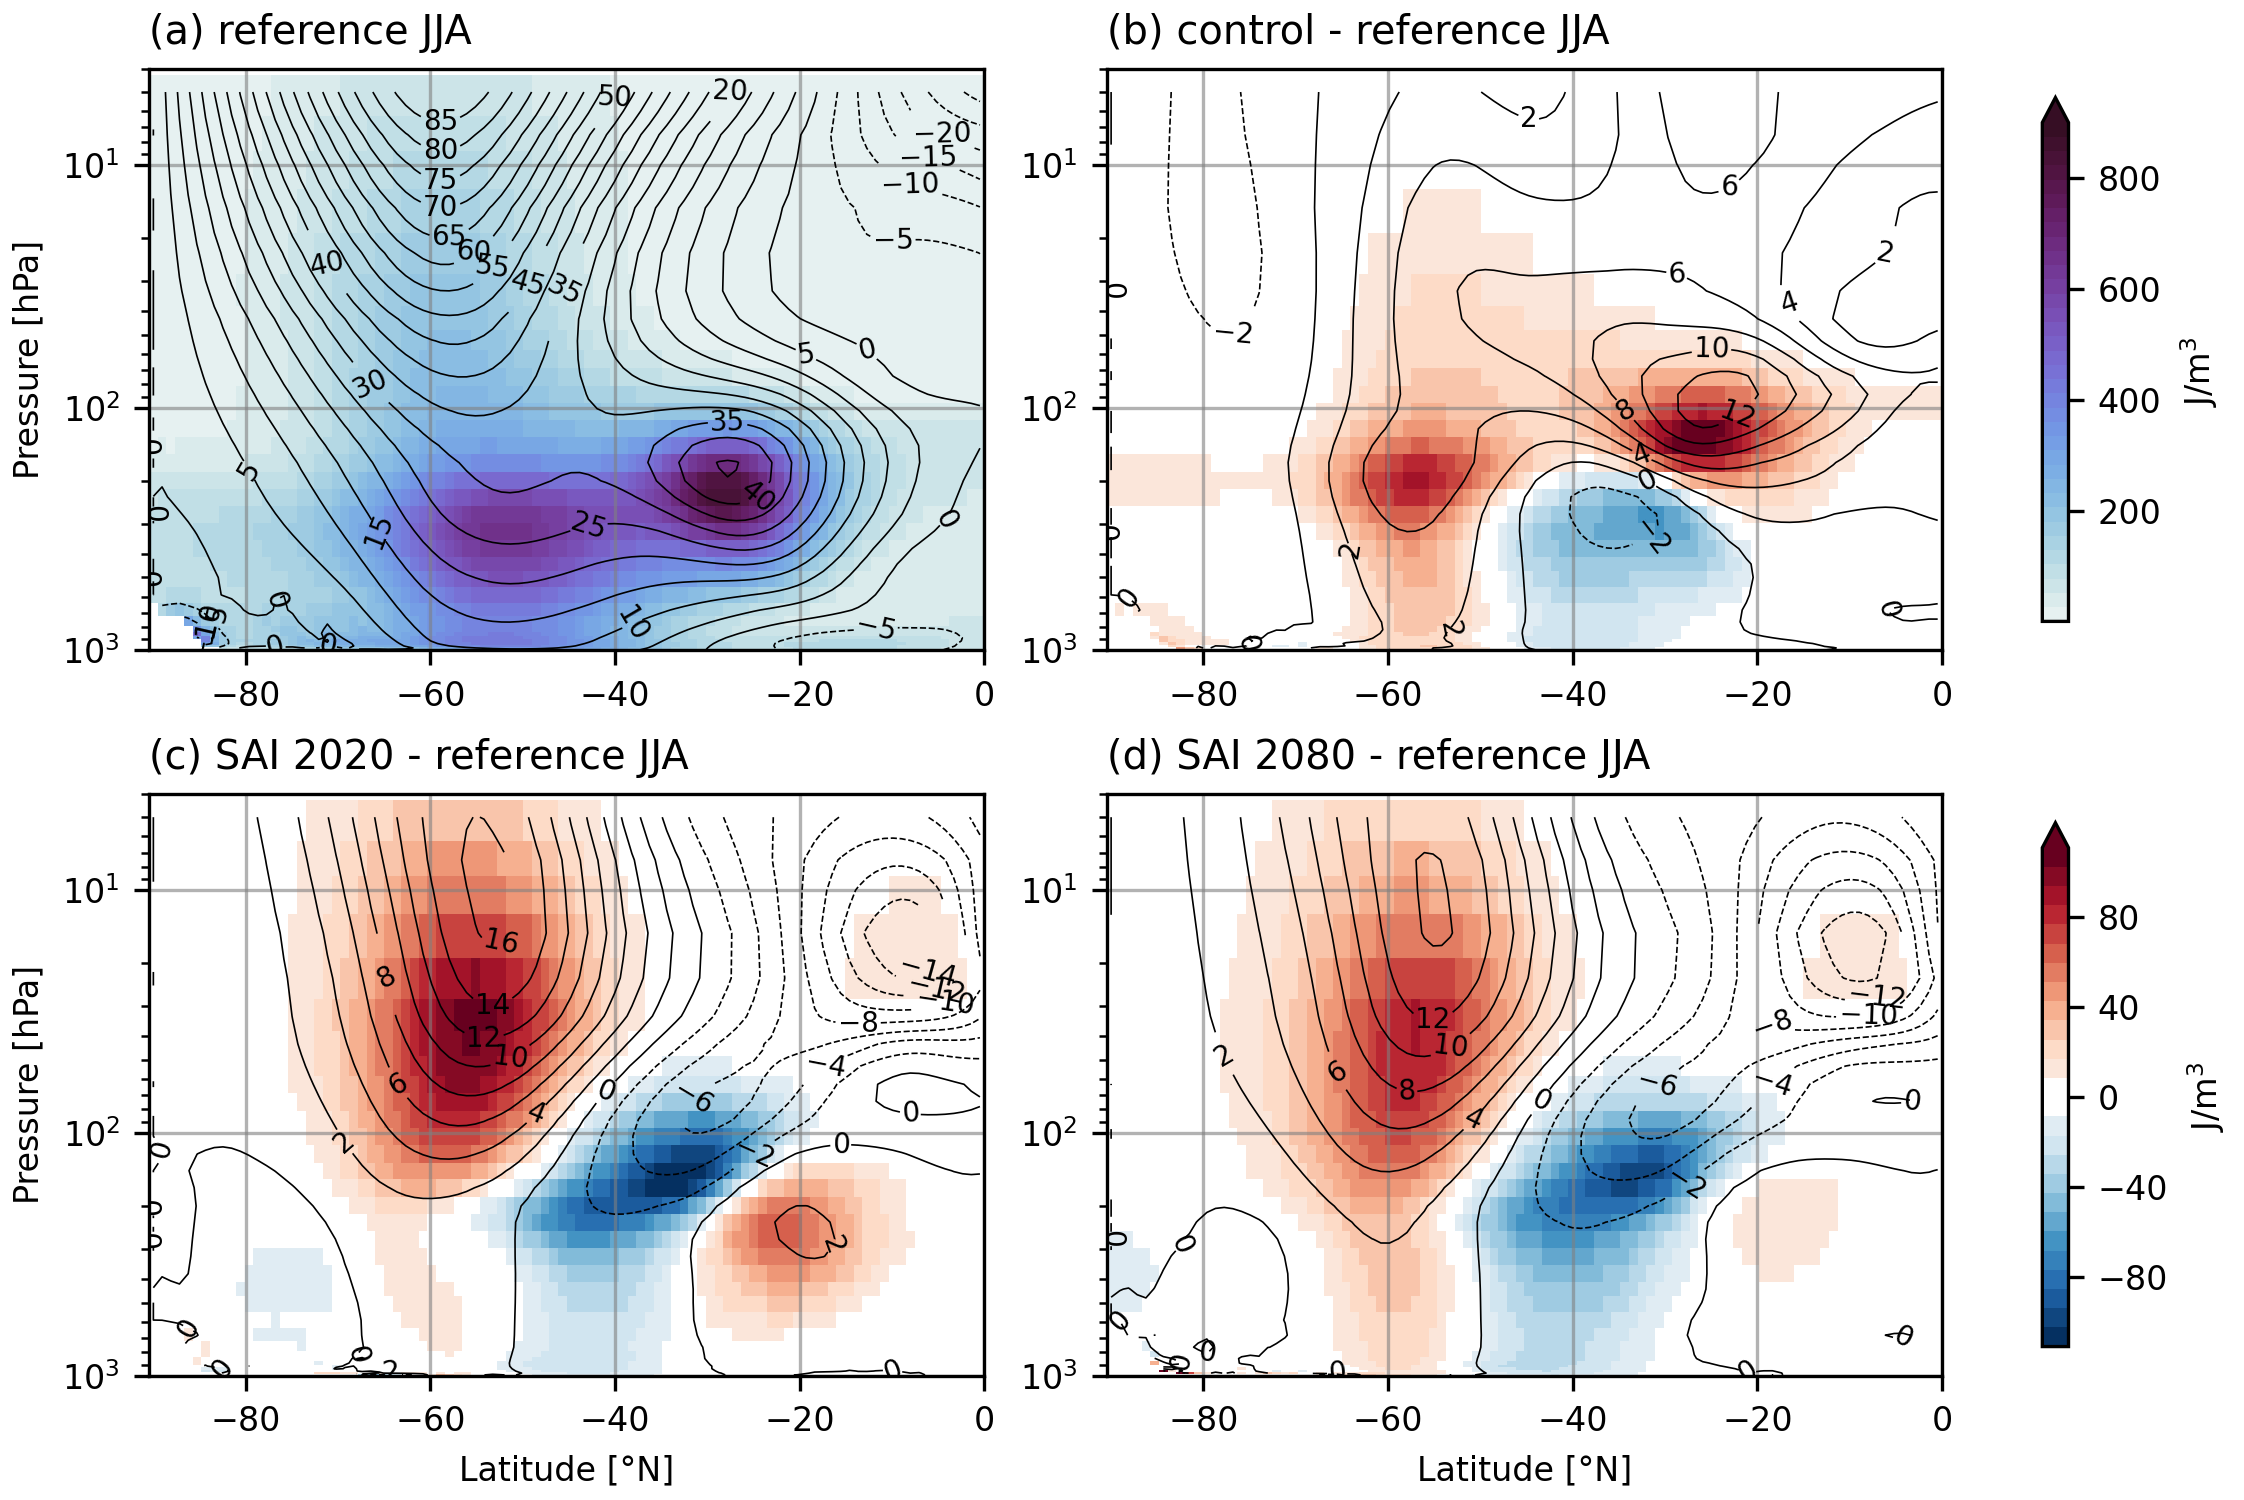
\includegraphics[width=0.95\linewidth]{images/KE_U_zmdiff_JJA.png}
	\caption{JJA mean zonal-mean kinetic energy (shading) and zonal-mean zonal wind (contours, m/s) for (a): Reference; (b-d): Control, SAI 2020 and SAI 2080 anomaly compared to Reference.}
	\label{fig:KE_U_zmdiff_JJA}
\end{figure}

